\begin{block}{Model: a stochastic game between the system and the crowd.}
  \begin{itemize}
    \item The game starts with the system receiving input $\bx$ and ends when the system turns in a set of labels $\by = (y_1, \ldots, y_n)$. 
    \item During the system's turn, the system may choose a query action $q \in \{1, \ldots, n\}$ to ask the crowd to label $y_q$. The system may also choose 
the wait action ($q = \acwait$) to wait for the crowd to respond to a pending query
or
the return action ($q = \acret$) to terminate the game and return its prediction given responses received thus far.
\item
The system can make as many queries in a row (i.e.\ simultaneously) as it wants, before deciding to wait or turn in.
\item When the wait action is chosen, the turn switches to the crowd, which provides a response $r$ to one pending query, and advances the game clock by the time taken for the crowd to respond. The turn then immediately reverts back to the system.
\item When the game ends (the system chooses the return action), the system evaluates a utility that depends on the accuracy of its prediction,
the number of queries issued and the total time taken.
\item The system should choose query and wait actions to
maximize the utility of the prediction eventually returned.
\item \textbf{Utility} trades off the accuracy of the MAP estimate according to the model's best guess of $\by$ incorporating all responses received by time $\tau$ and the cost of making queries: a (monetary) cost $\weightmoney$ per query made and penalty of $\weighttime$ per unit of time taken.
\begin{align}
  \label{eqn:utility}
  U(\sigma) &\eqdef \text{ExpAcc}(p(\by \given \bx, \bq, \bs, \br, \bt)) - (n_\text{Q} \weightmoney + \now \weighttime), \\
  \text{ExpAcc}(p) &= \E_{p(\by)}[\text{Accuracy}(\arg\max_{\by'} p(\by'))],
\end{align}
\item \textbf{Environmnet model}
\begin{align}
  \label{eqn:dynamics}
%p(\by, \br, \bt \mid \bx, \bq) \eqdef \p(\by \given \bx) \prod_{i=1}^k \presp(r_i \mid \bx, \by, q_i) \ptime(t_i \mid \bx, \by, q_i, s_i).
p(\by, \br, \bt \given \bx, \bq, \bs) \eqdef \p(\by \given \bx) \prod_{i=1}^k \presp(r_i \mid y_{q_i}) \ptime(t_i \mid s_i).
\end{align}

  \end{itemize}
\end{block}

\begin{block}{}
  \begin{center}
    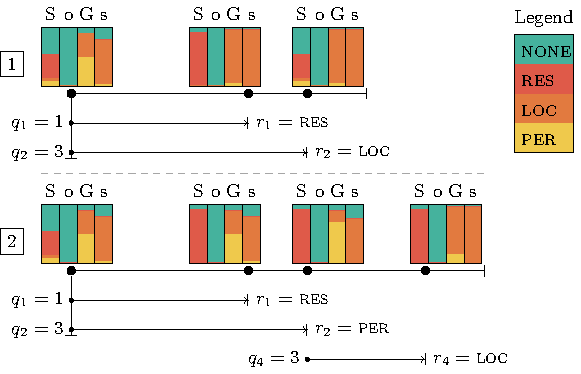
\includegraphics[width=0.59\columnwidth]{behavior}
    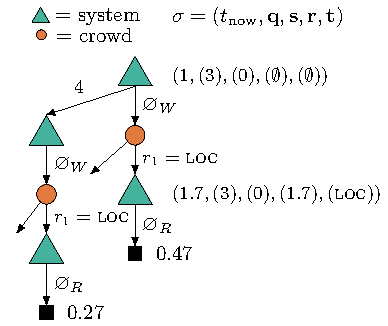
\includegraphics[width=0.39\columnwidth]{mcts_simple}
  \end{center}
\end{block}

\begin{block}{Learning and inference}
  \begin{itemize}
    \item TODO insert algorithm.
  \end{itemize}
\end{block}


\vfill

